\documentclass[10pt,a4paper]{article}
\usepackage[bindingoffset=0.2in,%
            left=2.5cm,right=2cm,top=2.7cm,bottom=1in,%
            footskip=.25in]{geometry}
\usepackage[utf8]{inputenc}
\usepackage[ngerman]{babel}
\usepackage{amsmath, amsfonts, amssymb}
\usepackage{scrpage2}
\usepackage{color}
\usepackage{titlesec}
\pagestyle{scrheadings}
\usepackage{ulem, contour}
\usepackage{multicol}
\usepackage{hyperref}
\usepackage{pdfpages}
\usepackage{tabularx}
\usepackage{subcaption, float}
\usepackage{scrextend}
\usepackage{enumerate, enumitem}
\usepackage[bottom, splitrule]{footmisc}
\usepackage{multirow}
\usepackage{csquotes}

\usepackage[style=authoryear, backend=biber]{biblatex}
\addbibresource{bibliography.bib}

\renewcommand{\ULdepth}{1.8pt}
\contourlength{0.8pt}

\newcommand{\cul}[1]{%
  \uline{\phantom{#1}}%
  \llap{\contour{white}{#1}}%
}

\graphicspath{
    {Images/}
}

\makeatletter
\newcommand*{\rom}[1]{\expandafter\@slowromancap\romannumeral #1@}
\makeatother

\newrobustcmd*{\parentexttrack}[1]{%
  \begingroup
  \blx@blxinit
  \blx@setsfcodes
  \blx@bibopenparen#1\blx@bibcloseparen
  \endgroup}

\AtEveryCite{%
  \let\parentext=\parentexttrack%
  \let\bibopenparen=\bibopenbracket%
  \let\bibcloseparen=\bibclosebracket}

\definecolor{gray}{rgb}{0.33, 0.33, 0.33}
\definecolor{greengreen}{rgb}{0.0, 0.56, 0.0}
\definecolor{fgreen}{rgb}{0.13, 0.55, 0.13}
\definecolor{grellow}{rgb}{0.68, 1.0, 0.18}
\definecolor{orange}{rgb}{1.0, 0.49, 0.0}
\definecolor{deepblue}{rgb}{0,0,0.5}
\definecolor{deepred}{rgb}{0.6,0,0}
\definecolor{deepgreen}{rgb}{0,0.5,0}

\usepackage{pifont}

\newcommand{\cmark}{\ding{51}}%
\newcommand{\xmark}{\ding{55}}%
\newcommand{\wontfix}{\rlap{$\square$}{\large\hspace{1pt}\xmark}}


\newcommand{\vnr}{31}
\newcommand{\anr}{1}

\ihead{}
\ohead{Anfängerpraktikum 2}
\chead{Versuch \vnr, Abgabe \anr : Licht- \& Signalgeschwindigkeit}
\cfoot{\pagemark}
\setheadsepline{.5pt}
\setlength\parindent{0pt}

\begin{document}

\begin{multicols}{2}
\begin{labeling}{Versuch-Nr.:}
\item[\textcolor{white}{x}Protokollant:\hspace{38pt}] \cul{Name} \wontfix
\item[\textcolor{white}{x}Zusammenarbeit\footnotemark mit:] \cul{Name} $\square$
\item[\textcolor{white}{x}Datum:\hspace{62pt}] \cul{\today}

\columnbreak

\item[Kurs: \hspace{27pt}] \cul{Anfängerpraktikum 2}
\item[Assistent: \hspace{8.7pt}] \cul{Name}
\item[Versuch-Nr.:] \underline{\vnr}
\end{labeling}
\end{multicols}

\begin{figure}[h]
\hspace{-0.5cm}\centerline{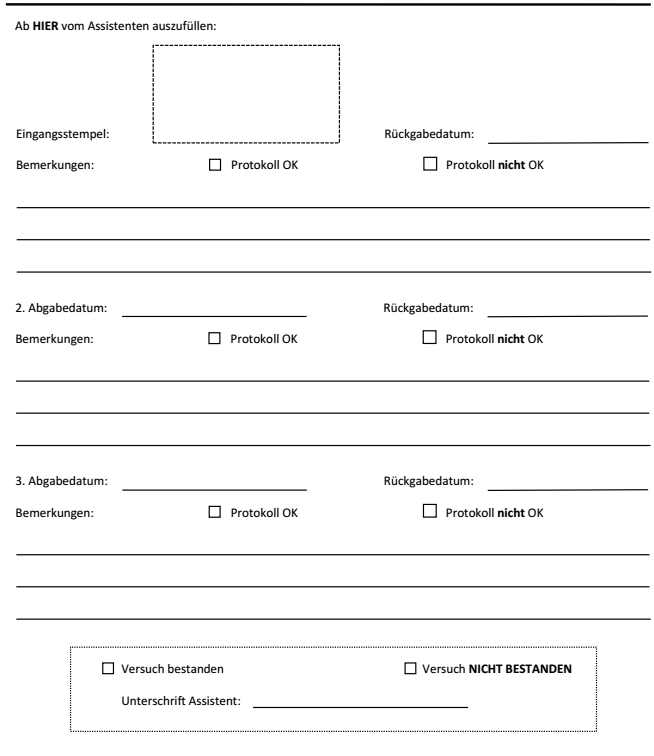
\includegraphics[width=1.1\linewidth , height=19cm]{Deckblatt_rest}}
\end{figure}

\newpage

\tableofcontents

\vspace{10pt}


\section{Aufgabenstellung}
\begin{flushleft}
Der Versuch \vnr behandelt das Ermitteln der Licht- und Signalgeschwindigkeit im Experiment. Dabei unterteilen wir diesen Versuch in zwei Teile.

\textbf{Teil \rom{1}}: Lichtgeschwindigkeit

Die Lichtgeschwindigkeit anahand der Laufzeit des Lichtes bei verschiedenen Strecken bestimmen.
\end{flushleft}
\begin{flushleft}
\textbf{Teil \rom{2}}: Signalgeschwindigkeit

Die Signaldauer in verschieden Langen Kabeln ermitteln und daraus die Signalgeschwindigkeit bestimmen.
\end{flushleft}

\subsection{Physikalischer Hintergrund}
\begin{flushleft}
Das Licht bewegt sich mit der Lichtgeschwindigkeit, die ca. $300\hspace{1pt}000 \frac{km}{s}$ beträgt. Licht ist dabei das schnellste \glqq Objekt\grqq.

Zusätzlich kann man die die Dielektrizitätszahl $\varepsilon_r$ von Signalleitern über die Signalgeschwindigkeit der elektromagnetischen Wellen im Kabel bestimmen. Diese gibt die relative Verringerung der Ausbreitungsgeschwindigkeit an.
\begin{equation}\label{eq:diel}
v = \frac{1}{\sqrt{\varepsilon_r}} c_0
\end{equation}
\end{flushleft}

\subsection{Verifikation der Wellengleichung}
\begin{flushleft}
Bevor wir den Versuch durchführen wollen wir zunächst die Wellengleichung verifizieren.

Die Wellengleichung ist beschrieben durch
\begin{equation}\label{eq:welle}
\frac{\partial^2 U}{\partial x^2} = \frac{1}{v^2} \frac{\partial^2 U}{\partial t^2}
\end{equation}
Die Lösungsfunktionen sind angegeben durch
\begin{equation}\label{eq:wloes}
U(x, t) = U_1(x - vt) + U_2 (x + vt)
\end{equation}
Wir setzen die Lösung nun in die Wellengleichung ein, um sie zu verifizieren:
\begin{align*}
\frac{\partial^2}{\partial x^2} U_1(x - vt) + U_2 (x + vt) &= \frac{1}{v^2} \frac{\partial^2}{\partial t^2} U_1(x - vt) + U_2 (x + vt) \\
U_1^{''}(x - vt) + U_2^{''}(x - vt) &= \frac{1}{v^2} (U_1^{''}(x - vt)v^2 + U_2^{''}(x - vt)v^2) \\
U_1^{''}(x - vt) + U_2^{''}(x - vt) &= U_1^{''}(x - vt) + U_2^{''}(x - vt) \\
0 &= 0
\end{align*}
Wir haben somit die Wellengleichung verifiziert.
\end{flushleft}

\section{Messmethoden}
\begin{flushleft}
Für diesen Versuch erzeugen wir ein Signal mit einem \textit{Signalgenerator} und senden dieses für Teil \rom{1} an eine LED, die Licht zu einem Reflektor ausstrahlt, der das Signal dann an eine Leuchtdiode reflektiert und für Teil \rom{2} durch ein Kabel und in beiden Fällen zurück zu einem Oszillator. Wir können so durch die Intensitätsschwankungen des Lichtes die Zeit bestimmen, die das Licht für die Strecke benötigt.
\end{flushleft}

\subsection{Versuchsaufbau \& -durchführung}
\begin{flushleft}
\begin{figure}[H]
\centering
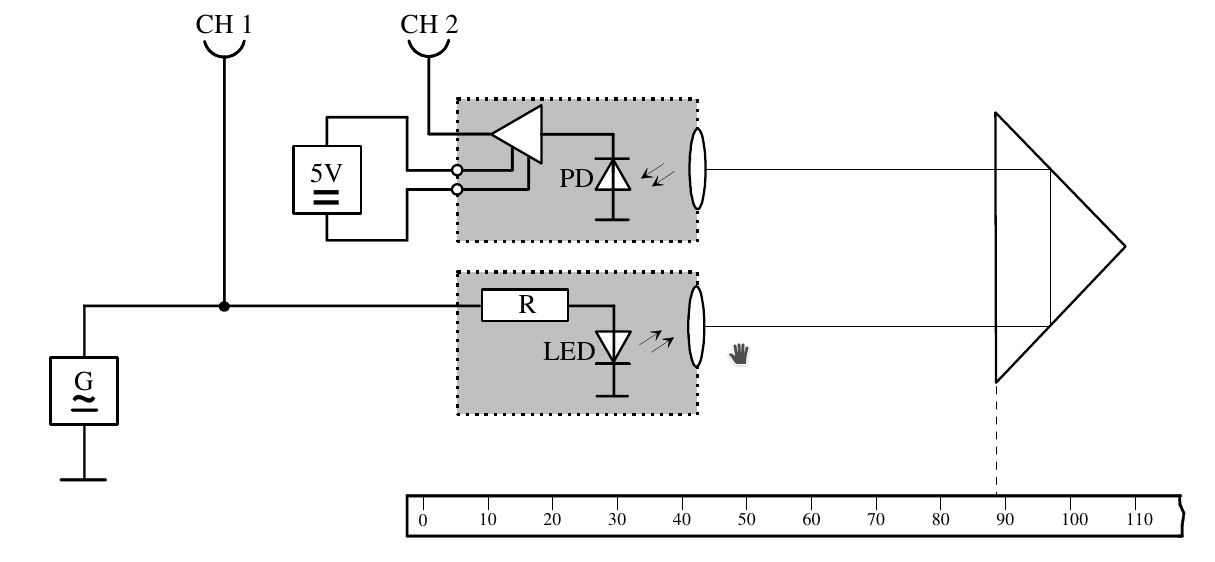
\includegraphics[scale=0.4]{schaltbild_licht}
\caption{Schaltbild zur Bestimmugn der Lichtgeschwindigkeit (Teil \rom{1}).}
\label{fig:licht}
\end{figure}
Die Abbildung \ref{fig:licht} zeigt den Aufbau zur Bestimmung der Lichtgeschwindigkeit.
\begin{itemize}
\item G = Signalgenerator
\item CH1 / CH2 = Kanal 1 / 2 Oszilloskop
\end{itemize}
Die dünne Linie in der Abbildung zeigt den Weg des Lichtes.

\vspace{4pt}

Für \textbf{Teil \rom{2}} verbinden wir \textit{CH1} sowie \textit{CH2} mit dem jeweiligen Kabel und hängen hinter \textit{CH2} einen Widerstand von $R = 50 \Omega$.
\end{flushleft}

\section{Versuchsergebnisse und Diskussion}
\begin{flushleft}
\textbf{Teil \rom{1}}
\begin{figure}[H]
\centering
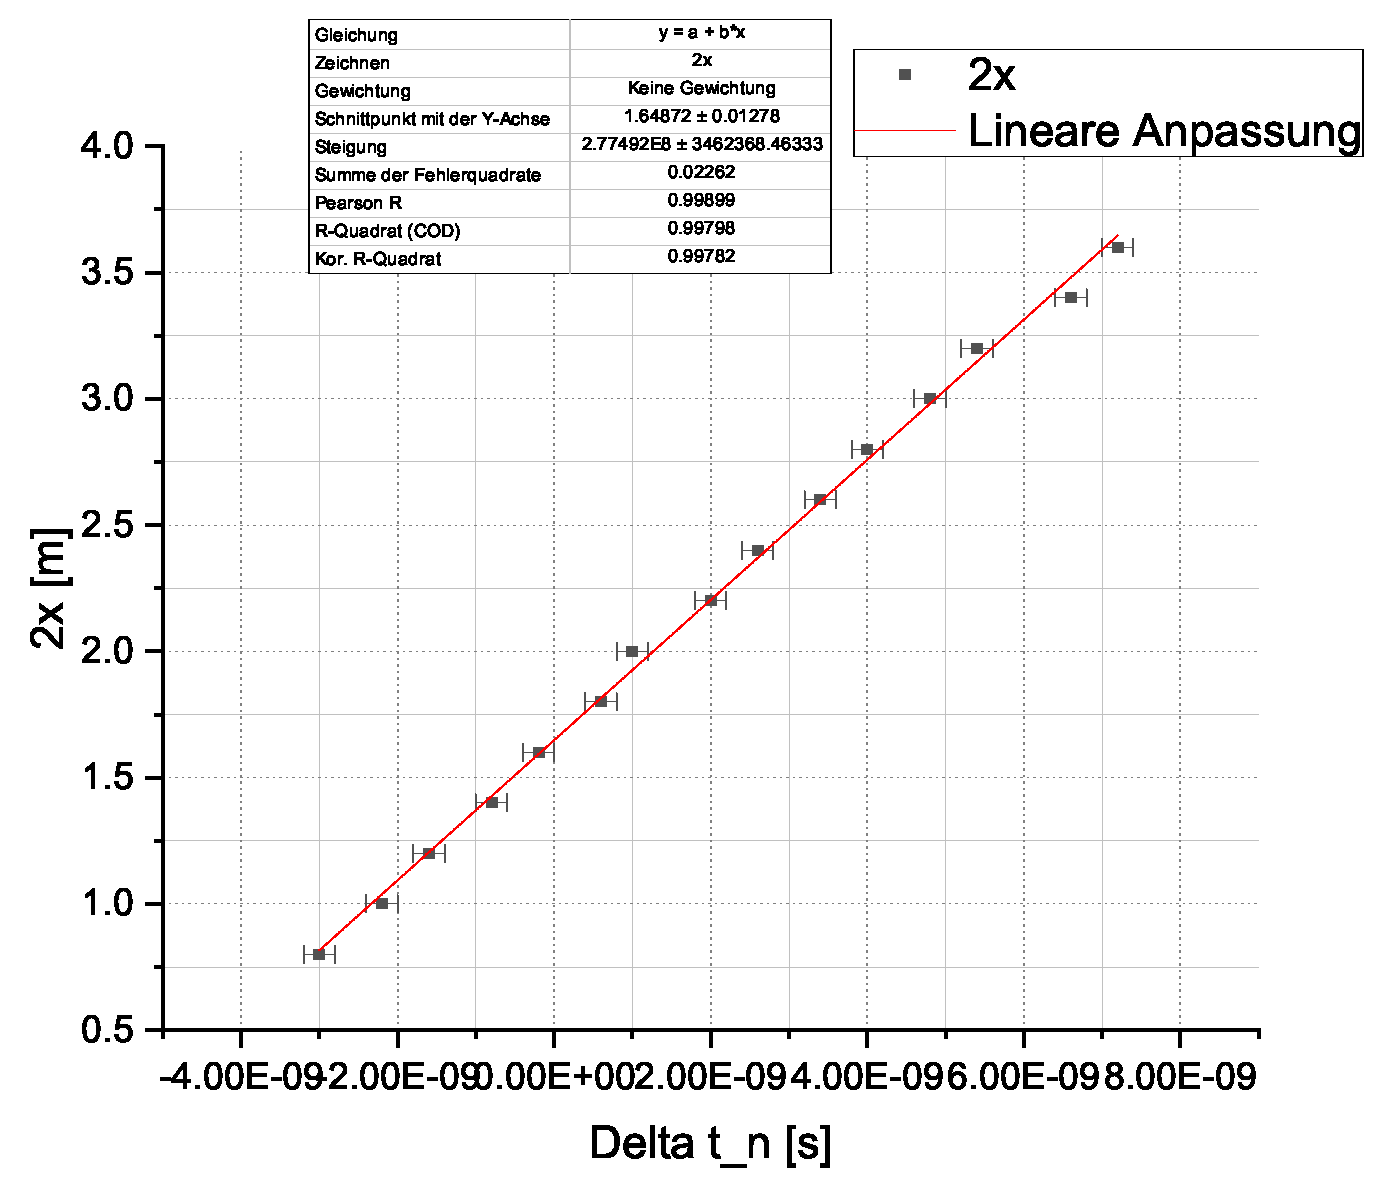
\includegraphics[scale=0.45]{Reflektor}
\caption{Laufzeiten des Lichtes.}
\label{fig:refl}
\end{figure}

Aus den Messdaten können wir nun die Lichtgeschwindigkeit bestimmen. Die lineare Regression ergibt dabei $(277.492 \pm 0.346) \cdot 10^6 \frac{m}{s}$ für die Lichtgeschwindigkeit.

Der Literaturwert der Lichtgeschwindigkeit beläuft sich auf $299\hspace{1pt}792\hspace{1pt}458 \frac{m}{s}$. DEr von uns ermittelte Wert weicht um rund $22.3 \cdot 10^6 \frac{m}{s}$ bzw. $7.44\%$ ab. Diese Abweichung ist sehr wahrscheinlich durch äußere Einflüsse verursacht.

\vspace{8pt}

\textbf{Teil \rom{2}}
\begin{figure}[H]
\centering
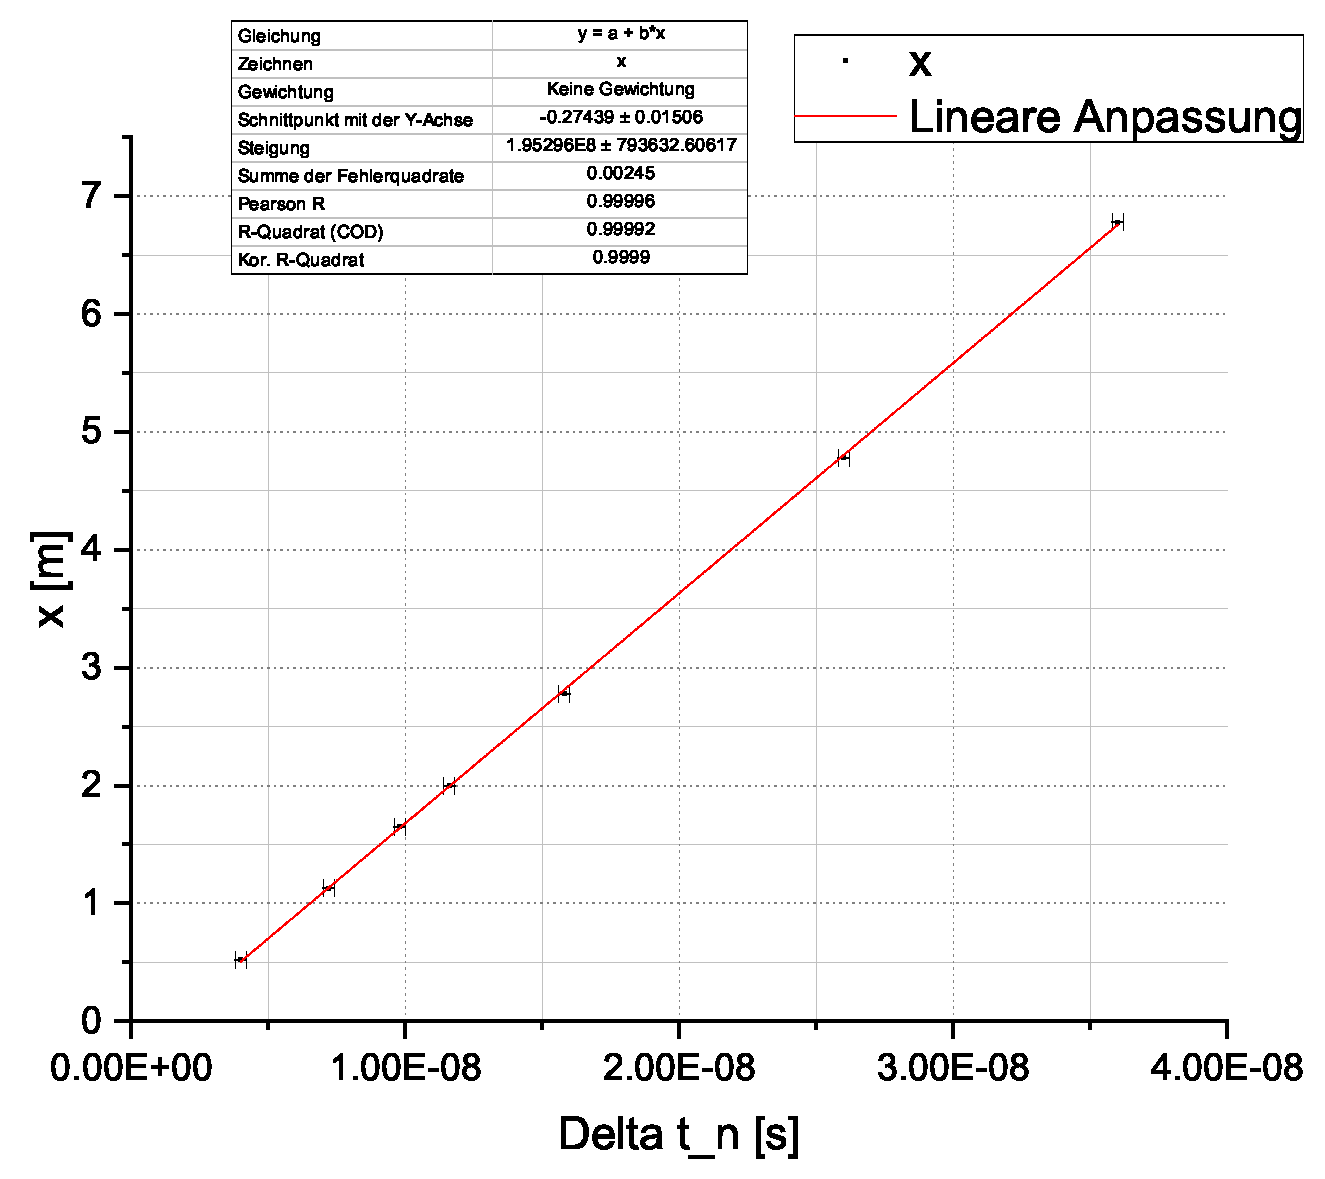
\includegraphics[scale=0.45]{Kabel}
\caption{Signallaufzeiten der Kabel.}
\label{fig:kab}
\end{figure}
Aus der Linearen Regression können wir die Signalgeschwindigkeit $c$ des Kabels bestimmen. Die Signalgeschwindigkeit des verwendeten Kabels haben wir somit auf $(195.296 \pm 0.794) \cdot 10^6 \frac{m}{s}$. Ein Koaxialkabel besitzt dabei typischerweise eine Signalgeschwindigkeit von rund $200\hspace{1pt}000 \frac{km}{s}$; somit ist unser Ergebnis ziemlich genau. Die Abweichung beträgt rund $4.7 \cdot 10^6 \frac{m}{s}$ ($2.35\%$).

Mit diesem ermittelten Wert können wir nun die Dielektrizitätszahl $\varepsilon_r$ des Kabels bestimmen (Gleichung \ref{eq:diel}, v = c).
\begin{align*}
\varepsilon_r &= \frac{c_0}{v}^2 = \frac{c_0}{195.296 \cdot 10^6 \frac{m}{s}}^2 \approx 2.356 \\
\Delta \varepsilon_r &= |- c_0^2 \cdot \frac{2 \cdot \Delta v}{(v^2)^2}| = |- c_0^2 \cdot \frac{2 \cdot 0.794 \cdot 10^6}{((195.296 \cdot 10^6)^2)^2}| \approx 0.98 \cdot 10^{-10} \approx 1 \cdot 10^{-9}
\end{align*}
\end{flushleft}

\section{Fazit}
\begin{flushleft}
Der Versuch \vnr\hspace{1pt} hat gezeigt, dass das Ermitteln der Lichtgeschwindigkeit durchaus komplex ist.
\end{flushleft}

\begingroup
\raggedright
\sloppy
\printbibliography[heading=bibintoc,title={6 \hspace{6pt} Literatur}]
\endgroup

\newpage

\section{Appendix: Rohdaten}
\begin{flushleft}
Anbei sind die Rohdaten (Signalverläufe) für diesen Versuch beigelegt. Die ersten Signalverläufe (wohlgeformter Sinus) sind dabei die Verläufe zur Messung mit der Photodiode, die restlichen sind zu der Messung mit Kabel (mit \textit{BNC-KABEL} beschriftet). Es ist zu beachten, dass für die Messungen mit der Photodiode der Wert von $x$ die \textbf{einfache Weglänge} beschreibt (wir senden das Licht aber zu einem Reflektor und zurück - Siehe Abbildung \ref{fig:licht} zum Versuchsaufbau).
\end{flushleft}

\includegraphics[page=1, scale=0.45]{Anhang_Rohdaten}

\includegraphics[page=2, scale=0.45]{Anhang_Rohdaten}

\includepdf[pages=3-, nup=1x3, width=.9\textwidth, pagecommand={}]{Anhang_Rohdaten}
\end{document}